\section{Introduction}\label{sec:intro}

Let $(a_1,\dots a_n)$ be a point array in a metric space $X$ and $T$ be a 
tree with the vertexes labeled by $\{a_1,\dots,a_n\}$.
We say that $(a_1,\dots a_n)$  satisfies $T$-tree comparison if there is a point array $(\~a_1,\dots, \~a_n)$ in the Hilbert space $\HH$ such that 
\[|\~a_i-\~a_j|\ge|a_i-a_j|\]
for any $i$ and $j$ and the equality holds if for every edge $(i,j)$ in $T$.

We say that a metric space $X$ satisfies $T$-tree comparison if 
every $n$-points arrays in $X$ satisfies the $T$-tree comparison.
We say that  $X$ satisfies all tree comparison
If $X$ satisfies $T$-tree comparison for all trees $T$ then we say that 

\begin{comment}
\begin{wrapfigure}{r}{20 mm}
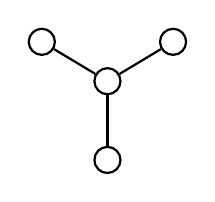
\begin{tikzpicture}[scale=1,
  thick,main node/.style={circle,draw,font=\sffamily\bfseries,minimum size=3mm}]

  \node[main node] (1) at (5/6,1) {};
  \node[main node] (2) at (0,3/2){};
  \node[main node] (3) at (10/6,3/2){};
  \node[main node] (4) at (5/6,0) {};

  \path[every node/.style={font=\sffamily\small}]
   (1) edge node[above]{}(2)
   (1) edge node[above]{}(3)
   (1) edge node[above]{}(4);
\end{tikzpicture}
\end{wrapfigure}
\end{comment}

\parbf{Monopolar comparison.}
For example, the (3+1)-comparison described in \cite{AKP} is $S_3$-tree comparison, where $S_3$ denotes the star-like tree as on the diagram.
Similarly, the ($n$+1)-comparison described in \cite{AKP} as $S_n$-tree comparison for the star-like tree $S_n$ with one vertex of degree $n$ and $n$ end-vertexes.
In these examples one vertex called \emph{pole} of the tree adjacent to all other vertexes,
by that reason we call it \emph{monopolar}.

In \cite[4.1]{AKP} it is proved that any Alexandrov space with nonnegative curvature satisfies the so called  ($n$+1)-comparison.
Using the tree comparison, the later statement can be reformulated the following way.
If a length-metric space satisfies $S_3$-comparison, then it also satisfies $S_n$-comparison for all integer $n$.

\parbf{Dipolar comparison.} 
A tree will be called \emph{dipoar} if it has exactly two poles;
that is, two vertexes of degree at least two.

In section ??? we will show that the comparison for the any Alexandrov space with nonnegative curvature satisfies the tree comparisons for the first two trees an the following diagram.

\begin{comment}
\begin{center}

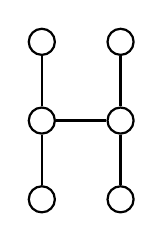
\begin{tikzpicture}[scale=1,
  thick,main node/.style={circle,draw,font=\sffamily\bfseries,minimum size=3mm}]

  \node[main node] (1) at (0,0) {};
  \node[main node] (2) at (0,1){};
  \node[main node] (3) at (0,2){};
  \node[main node] (4) at (1,0) {};
  \node[main node] (5) at (1,1) {};
  \node[main node] (6) at (1,2) {};

  \path[every node/.style={font=\sffamily\small}]
   (1) edge node[above]{}(2)
   (2) edge node[above]{}(3)
   (2) edge node[above]{}(5)
   (4) edge node[above]{}(5)
   (5) edge node[above]{}(6);
\end{tikzpicture}
\hskip10mm
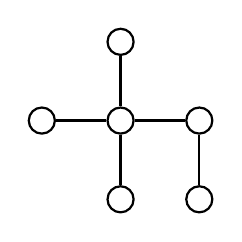
\begin{tikzpicture}[scale=1,
  thick,main node/.style={circle,draw,font=\sffamily\bfseries,minimum size=3mm}]

  \node[main node] (1) at (0,1) {};
  \node[main node] (2) at (1,0){};
  \node[main node] (3) at (1,1){};
  \node[main node] (4) at (1,2) {};
  \node[main node] (5) at (2,0) {};
  \node[main node] (6) at (2,1) {};

  \path[every node/.style={font=\sffamily\small}]
   (1) edge node[above]{}(3)
   (2) edge node[above]{}(3)
   (3) edge node[above]{}(6)
   (4) edge node[above]{}(3)
   (5) edge node[above]{}(6);
\end{tikzpicture}
\hskip10mm
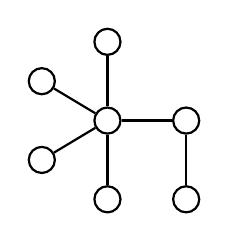
\begin{tikzpicture}[scale=1,
  thick,main node/.style={circle,draw,font=\sffamily\bfseries,minimum size=3mm}]

  \node[main node] (0) at (1/6,1/2) {};
   \node[main node] (1) at (1/6,3/2) {};
  \node[main node] (2) at (1,0){};
  \node[main node] (3) at (1,1){};
  \node[main node] (4) at (1,2) {};
  \node[main node] (5) at (2,0) {};
  \node[main node] (6) at (2,1) {};

  \path[every node/.style={font=\sffamily\small}]
     (0) edge node[above]{}(3)
   (1) edge node[above]{}(3)
   (2) edge node[above]{}(3)
   (3) edge node[above]{}(6)
   (4) edge node[above]{}(3)
   (5) edge node[above]{}(6);
\end{tikzpicture}

\end{center}
\end{comment}

In section ??? we will show that the comparison for the third tree on the diagram implies
the curvature condition introduced by Ma--Trudinger--Wang (briefly MTW condition) and convexity of tangent injectivity loci (briefly CTIL condition).
These two conditions appear in the study of contunuity of optimal transport betweens regular measures with positive continuous density functions.
(The continuity implies both MTW and CTIL conditions and slightly stronger version of these two conditions imply the continuity;
see \cite{FRV-Nec+Suf} \cite{MTW+CTIL} and the references there in.)

Note that dipolar comparison provides a uniform way to treat combined CTIL+MTW condition;
this partially answers the question of Cédric Villani in ???.

\parbf{Polypolar comparison.}
In Section~\ref{sec:all-tree} we show that if the space satisfies all tree comparisons then it is isometric to a quotient space of a subset in Hilbert space by an isometric group action.

Any quotient of Hilber space by a group of isometries is an Alexandrov space with nonnegative curvature.
In particular, all tree comparisons provides a sufficient condition on $n$-point metric spaces which admit an isometric embedding into an Alexandrov space with nonnegative curvature.
For $n\le 5$ this condition is also sufficient, likely it is also sufficient for $n=6$, but it is not sufficient for $n\ge 7$.
